%!TEX root = ../dissertation.tex

\chapter{Results and Discussion}
\label{cha4:results}

\section{Simulator}
As it was specified on Figure \ref{cha1:sec1:fig:curr_eye_model}, the current eye prototype contains a baseline length of $53.7 \ mm$ on the torsional axis. To make the comparisons easier, this baseline was also used in the simulator.
\subsection{Rotation estimation error}
\label{reiovniorevn}
On experiment 1, the variance used on the Gaussian distribution was $4 \degree$ so to simulate the saccade amplitudes of the human eye. On experiment 2, the variance was $15 \degree$, in order to understand how the estimation algorithm works in wider amplitude ranges.
The lines on each graph represent the best fitting of the points.
\subsubsection{Simulation Parameters}
The following parameters were used to run the simulation. Zmax and Zmin refer to the range in which points are simulated explained on section \ref{rienreive}.
\begin{itemize}
	\item Maximum Matches : $30$
	\item False Matches : $10 \%$ of maximum matches
	\item Good Matches : $50 \%$ of the maximum matches
	\item Gaussian Noise $\sigma^2$ : $10 \ px$
	\item Number of saccades: $45$
	\item Zmin : $0.05 m$
	\item Zmax : $5 m$
\end{itemize}
\subsubsection{Experiment 1 - Saccade amplitudes generated with $\sigma^2 = 4 \degree $}
Figures \ref{cha5:sec1:10anglex}, \ref{cha5:sec1:10angley} and \ref{cha5:sec1:10anglez}, show the error, computed as \ref{firenr}, from the estimation of the rotation per saccade amplitudes on the horizontal, vertical and torsional axis, respectively. The amplitudes were generated randomly around a specific axis in a normal distribution with variance $\sigma^2 = 4 \degree$. Table \ref{cha5:sec1:10angleaxist}, shows the corresponding mean error in degrees per axis for each of the methods.

\begin{minipage}{0.33\textwidth}
	\centering
	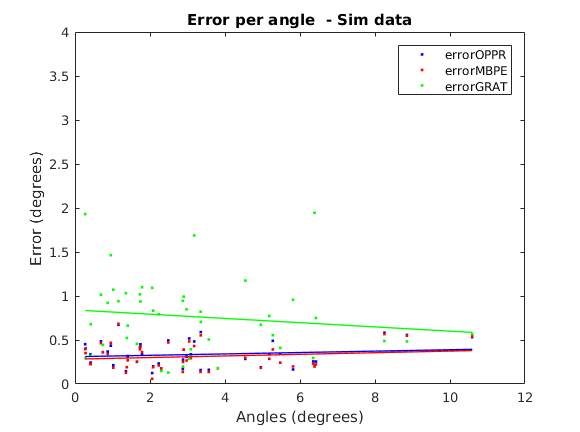
\includegraphics[width=\textwidth]{images/sim/10anglex.png}
	\captionof{figure}{Error per saccade amplitude (in degrees) under simulation on the horizontal axis.}
	\label{cha5:sec1:10anglex}
\end{minipage}
\begin{minipage}{0.33\textwidth}
	\centering
	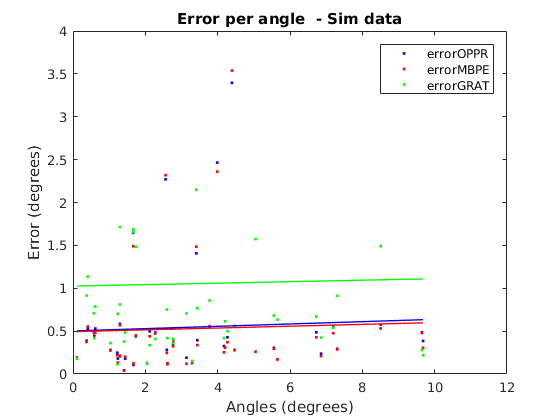
\includegraphics[width=\textwidth]{images/sim/10angley.png}
	\captionof{figure}{Error per saccade amplitude (in degrees) under simulation on the vertical axis.}
	\label{cha5:sec1:10angley}
\end{minipage}
\begin{minipage}{0.33\textwidth}
	\centering
	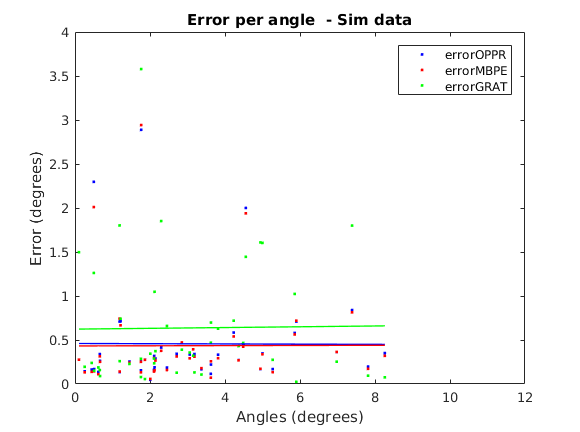
\includegraphics[width=\textwidth]{images/sim/10anglez.png}
	\captionof{figure}{Error per saccade amplitude (in degrees) under simulation on the torsional axis.}
	\label{cha5:sec1:10anglez}
\end{minipage}
\begin{table}
	\centering
	\begin{tabular}{| l | l | l | l |}
		\hline
		Method & X Mean & Y Mean & Z Mean \\
		\hline
		OPPR &  0.33 \degree & 0.54 \degree & 0.46 \degree \\
		\hline
		MBPE &  0.31 \degree & 0.52 \degree & 0.44 \degree\\
		\hline
		GRAT &  0.77 \degree & 1.05 \degree & 0.64 \degree\\ 
		\hline
	\end{tabular}
	\captionof{table}{Mean error (in degrees) per method and per axis.}
	\label{cha5:sec1:10angleaxist}
\end{table}		

Figure \ref{cha5:sec1:10angle} shows the error from the estimation of the rotation per saccade amplitudes randomly executed around all axis simultaneously. Table \ref{cha5:sec1:10anglet} shows the mean error and standard deviation for this experiment for each of the methods.

\begin{minipage}{0.5\textwidth}
	\centering
	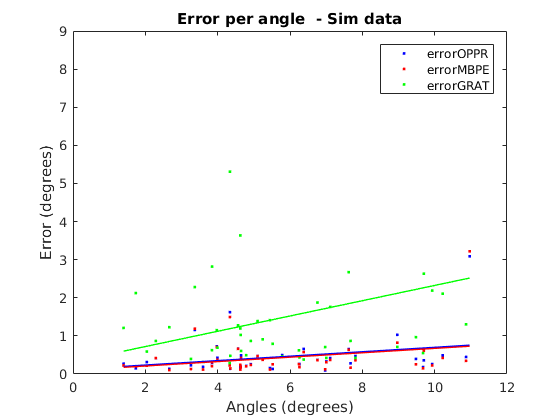
\includegraphics[width=\textwidth]{images/sim/10angle.png}
	\captionof{figure}{Error per saccade amplitude (in degrees) under simulation.}
	\label{cha5:sec1:10angle}
\end{minipage}
\begin{minipage}{0.5\textwidth}
	\centering
	\begin{tabular}{| l | l | l |}
			\hline
			Method & Mean & Standard Deviation \\
			\hline
			OPPR &  0.45 \degree & 0.49 \degree \\
			\hline
			MBPE &  0.42 \degree & 0.50 \degree \\
			\hline
			GRAT &  1.47 \degree & 1.76 \degree \\ 
			\hline
	\end{tabular}
	\captionof{table}{Mean error and standard deviation (in degrees) of the experiment on the left per each method tested}
	\label{cha5:sec1:10anglet}
\end{minipage}\\

Robust estimation was applied to filter out wrong matches and detected a $15.55 \%$ of them from the whole set of matches.

\subsubsection{Experiment 2 - Saccade amplitudes generated with $\sigma^2 = 15 \degree $}

Just like Experiment 1, Figure \ref{cha5:sec1:45angle} shows the error per  amplitude in degrees from random saccades around around all axis simultaneously, generated in a normal distribution with variance $\sigma^2 = 15 \degree $. Table \ref{cha5:sec1:45anglet} presents the respective mean error and standard deviation. Robust estimation detected a $ 22.55 \%$ of bad matches.

\begin{minipage}{0.5\textwidth}
	\centering
	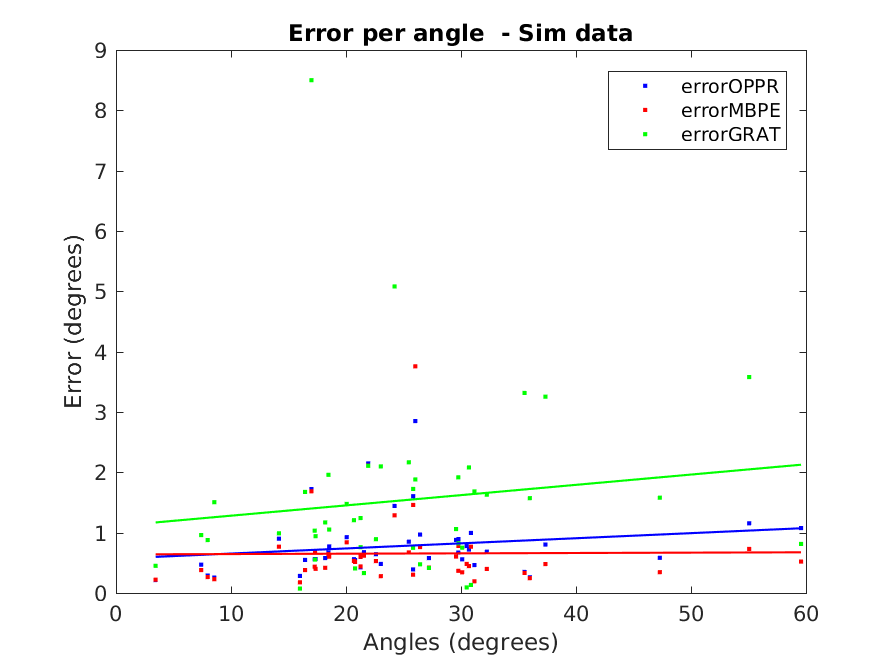
\includegraphics[width=\textwidth]{images/sim/45angle.png}
	\captionof{figure}{Error per saccade amplitude (in degrees) under simulation.}
	\label{cha5:sec1:45angle}
\end{minipage}
\begin{minipage}{0.5\textwidth}
	\centering
	\begin{tabular}{| l | l | l |}
		\hline
		Method & Mean & Standard Deviation \\
		\hline
		OPPR &  0.77 \degree & 0.49 \degree \\
		\hline
		MBPE &  0.65 \degree & 0.60 \degree \\
		\hline
		GRAT &  1.53 \degree & 1.43 \degree \\ 
		\hline
	\end{tabular}
	\captionof{table}{Mean error and standard deviation (in degrees) of the experiment on the left per each method tested}
	\label{cha5:sec1:45anglet}
\end{minipage}\\

\subsubsection{Overview}

Doing the saccades per isolated axis on Experiment 1, demonstrated that there is not a significant difference in the error around a specific coordinate by looking at Table \ref{cha5:sec1:10angleaxist}. Given that, the experiments can comfortably be executed with random saccades around all axis at the same time, which represents the real human eye more accurately.

Table \ref{cha5:sec1:10anglet} and Figure \ref{cha5:sec1:10angle} on Experiment 1, show that for angles under $ 12 \degree $ the mean error is under $0.5 \degree$ for the best two methods, \acrshort{oppr} and \acrshort{mbpe}, whereas for \acrshort{grat} the error is greater. \acrshort{mbpe} seems to be the best method in this case. However, the standard deviation is comparable to the mean for all the methods, alerting instability.

In Table \ref{cha5:sec1:45anglet} and Figure \ref{cha5:sec1:45angle} (Experiment 2), the conditions are all the same except for the amplitude range. Stil \acrshort{mbpe} and \acrshort{oppr} continue to thrive over \acrshort{grat}, this time having \acrshort{oppr} become worse as the saccade amplitude increases. This may be due to the fact that for a bigger saccade, the associated translation creates a larger effect that is not counter acted when using \acrshort{oppr}. Overall, the error increases as the saccade amplitude increases proportionally for all methods.

There might be several reasons as to why \acrshort{grat} performs worst than the other algorithms. Because the baseline length is small, the skew translation matrix, that generates the essential matrix together with the rotation, expressed in \ref{sec2:eq:fundm3}, will have values very close to zero, that during intermediate calculus in the minimization can reduce the accuracy of the estimation. Other reason could be that, because the depth, $\lambda$, is not being estimated, opposite to \acrshort{mbpe} (see \ref{fiorenfe}), the leeway to estimate the rotation is reduced, ending up with a poorer guess.
 

\subsection{Variable noise}
To test how Gaussian noise affects the algorithms, all the same parameters as the previous section were kept and the amplitude of the saccades was set to a variance of $4 \degree$, while the added noise varies from $0$ to $100 \ px$. 
\subsubsection{Simulation Parameters}
\begin{itemize}
	\item Maximum Matches : $30$
	\item Good Matches : $50 \%$ of the maximum matches
	\item False Matches : $10 \%$ of maximum matches
	\item Noise $\sigma^2$ : $0-100 \ px$ incrementing $10 \ px$ per iteration
	\item Number of saccades: $45$
	\item Zmin : $0.05 m$
	\item Zmáx : $5 m$
	\item Saccade amplitude $\sigma^2 : 4 \degree $
\end{itemize}
\begin{figure}[ht]
	\centering
	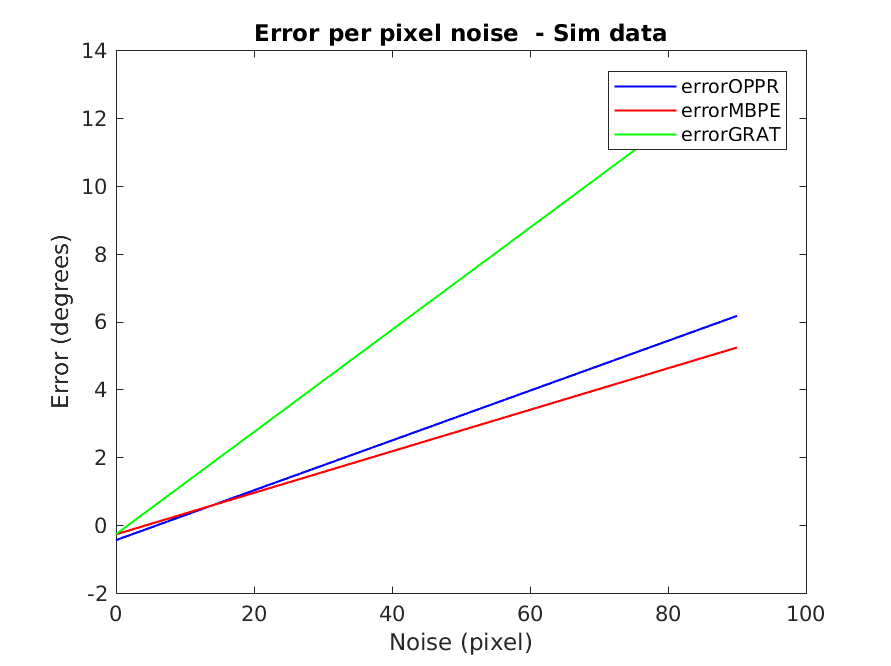
\includegraphics[width=0.5\textwidth]{images/sim/noise.png}
	\captionof{figure}{Error (in degrees) per Gaussian noise in the simulated image (in pixels).}
	\label{cha5:sec1:noise}
\end{figure}

\subsection{Variable baseline}
\subsection{Variable depth}

\subsection{Effect of RANSAC}

\section{Real System}
\subsection{Rotation estimation error}
The lines on each graph represent the best fitting of the points.
\subsubsection{Data collection}
To test the algorithms under the real system, 10 images of a scenery, with the setup mentioned on \ref{cha4:sec3:eyescheme}, were took with and without a chessboard at the same time as the \acrshort{imu} collected the current orientation of the eye prototype, for each experiment. Joining the images/orientations with each other made up to 45 different saccades. The algorithms were then run with the following parameters.
\subsubsection{System Parameters}
\begin{itemize}
	\item Maximum Matches : $30$
	\item Good Matches : $50 \%$ of the maximum matches
	\item Zmin : $0.05 m$
	\item Zmáx : $5 m$
	\item Saccade amplitude : random
\end{itemize}
\subsubsection{Experiment 1}
In experiment 1, all the 45 rotations obtained from the ground truth were valid to be analyzed.\\
Figure \ref{cha5:sec1:r1angle} presents the error per saccade amplitude on the real system in degrees for the camera, and Figure \ref{cha5:sec1:r1angleimu} shows the same for the \acrshort{imu}. Table \ref{cha5:sec1:r1anglet} displays the corresponding mean error and standard deviation for each method and for the \acrshort{imu}.

Robust estimation applied to the images detected $ 94.96 \%$ of wrongly paired matches. 

\begin{minipage}{0.5\textwidth}
\centering
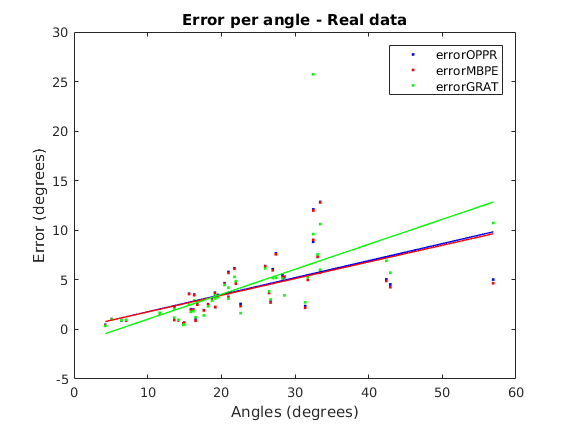
\includegraphics[width=\textwidth]{images/sim/r1angle.png}
\captionof{figure}{Error per saccade amplitude (in degrees) under the real system for the camera estimation.}
\label{cha5:sec1:r1angle}
\end{minipage}
\begin{minipage}{0.5\textwidth}
\centering
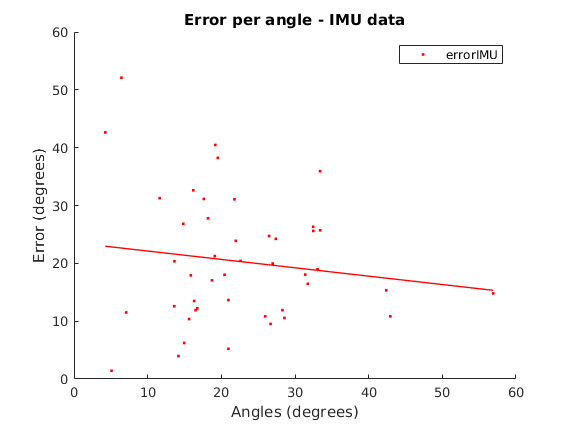
\includegraphics[width=\textwidth]{images/sim/r1angleimu.png}
\captionof{figure}{Error per saccade amplitude (in degrees) under the real system for the \acrshort{imu} estimation.}
\label{cha5:sec1:r1angleimu}
\end{minipage}\\

\begin{table}[ht]
	\centering
\begin{tabular}{| l | l | l |}
	\hline
	Method & Mean & Standard Deviation \\
	\hline
	OPPR &  3.90 \degree & 2.75 \degree \\
	\hline
	MBPE &  3.83 \degree & 2.75 \degree \\
	\hline
	GRAT &  4.13 \degree & 4.09 \degree \\ 
	\hline
	IMU &  20.34 \degree & 10.85 \degree \\ 
	\hline
	IMU without the vertical axis &  11.79 \degree & 3.57 \degree \\ 
	\hline
\end{tabular}
\captionof{table}{Mean error and standard deviation (in degrees) of the experiment on the left per each method tested}
\label{cha5:sec1:r1anglet}
\end{table}

\begin{figure}[ht]
	\centering
	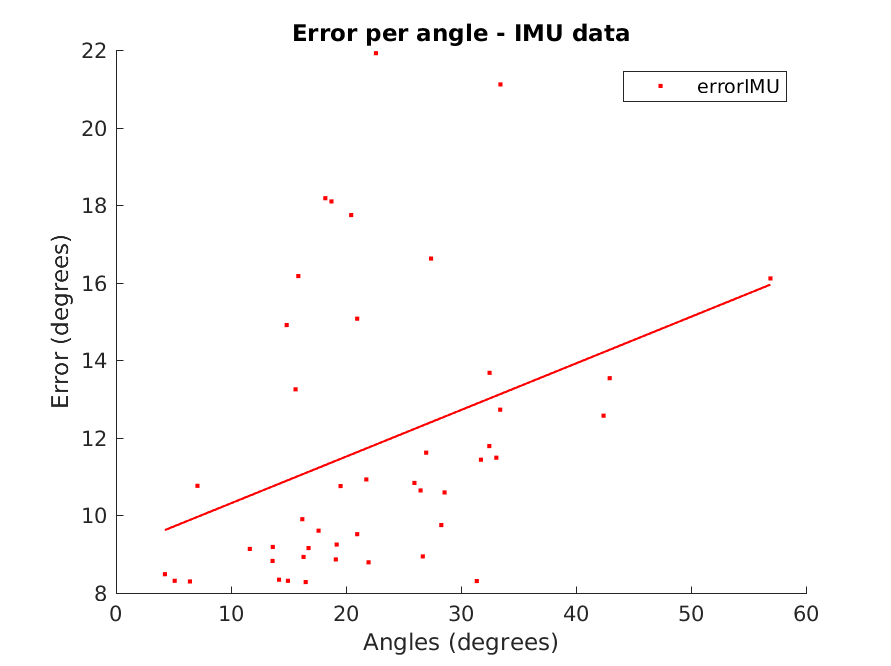
\includegraphics[width=0.5\textwidth]{images/sim/imuerrorissue.png}
	\captionof{figure}{The same experiment as \ref{cha5:sec1:r1angleimu} but only visualizing the error on the horizontal and torsional axis per saccade amplitude (in degrees).}
	\label{cha5:sec1:imuerrorissue}
\end{figure}


\subsubsection{Experiment 2}
In experiment 2, 13 of the saccades were invalid, thus only 32 are  assessed. Figure \ref{cha5:sec1:r2angle} and \ref{cha5:sec1:r2angleimu} exhibit the error per saccade amplitude in degrees for the camera estimation and for the \acrshort{imu} estimation, respectively. Table \ref{cha5:sec1:r2anglet} shows the corresponding mean error and standard deviation for each method and the \acrshort{imu}.

Robust estimation detected a $ 93.68 \%$ of bad matches.

\begin{minipage}{0.5\textwidth}
	\centering
	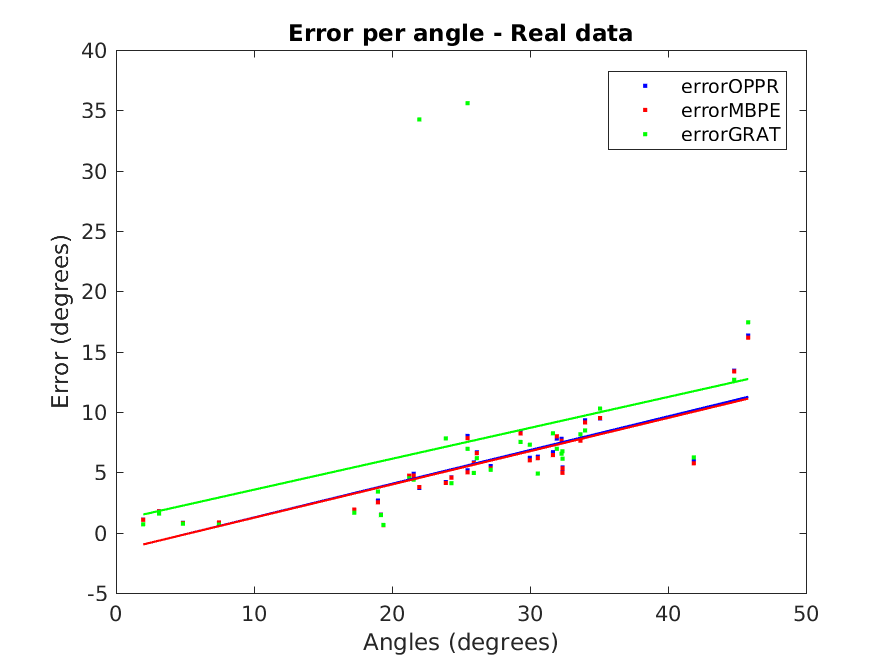
\includegraphics[width=\textwidth]{images/sim/r2angle.png}
	\captionof{figure}{Error per saccade amplitude (in degrees) under simulation for the camera estimation.}
	\label{cha5:sec1:r2angle}
\end{minipage}
\begin{minipage}{0.5\textwidth}
	\centering
	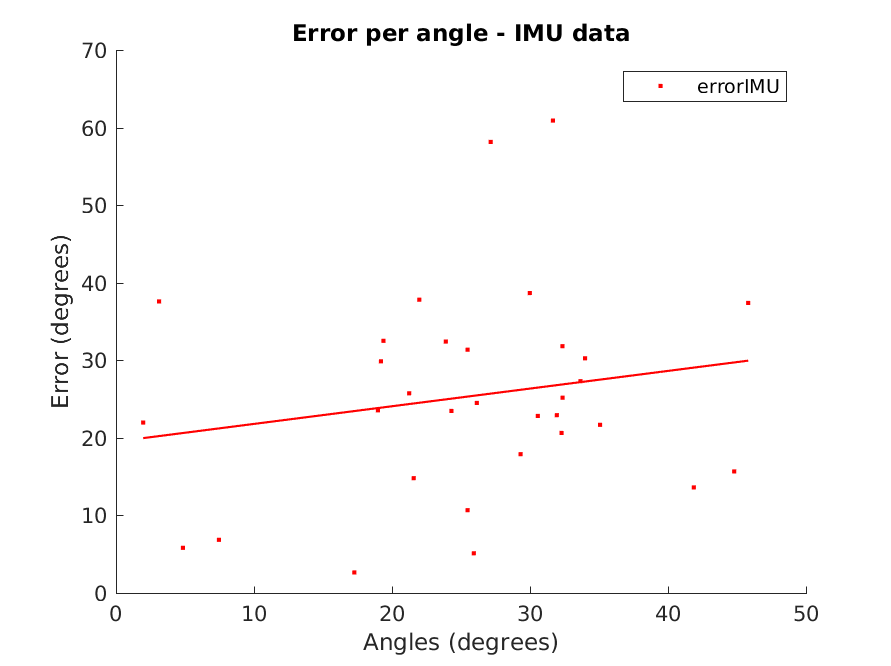
\includegraphics[width=\textwidth]{images/sim/r2angleimu.png}
	\captionof{figure}{Error per saccade amplitude (in degrees) under simulation for the \acrshort{imu} estimation.}
	\label{cha5:sec1:r2angleimu}
\end{minipage}\\

\begin{table}
	\centering
	\begin{tabular}{| l | l | l |}
		\hline
		Method & Mean & Standard Deviation \\
		\hline
		OPPR &  5.63 \degree & 3.43 \degree \\
		\hline
		MBPE &  5.55 \degree & 3.40 \degree \\
		\hline
		GRAT &  7.57 \degree & 7.79 \degree \\ 
		\hline
		IMU &  25.36 \degree & 13.13 \degree \\ 
		\hline
	\end{tabular}
	\captionof{table}{Mean error and standard deviation (in degrees) of the experiment on the left per each method tested}
	\label{cha5:sec1:r2anglet}
\end{table}

\subsubsection{Overview}

Both experiments were the same but with two different sets of images, in order to validate the results.

Similarly to the simulation results in section \ref{reiovniorevn}, as seen on Figures \ref{cha5:sec1:r1angle} and \ref{cha5:sec1:r2angle}, \acrshort{oppr} and \acrshort{mbpe} keep being better than \acrshort{grat}.

When comparing the camera estimation algorithms, in experiment 1, the best mean error for the camera is $3.83 \degree $, from \acrshort{mbpe} with a standard deviation of $2.75 \degree$. This error is probably due to noise in the image or even false matches that were not filtered out in the robust estimation. As it is real data, there is always noise associated and imposing stricter parameters for the quantity of good matches or maximum error for RANSAC (see section \ref{rnfireonce}) will eventually not yield enough point matches to work with.

Experiment 1's estimation errors are smaller than Experiment 2, that is because the points in 1 are more concentrated around smaller angles where the error is less.

The \acrshort{imu} estimation results, shown on Figures \ref{cha5:sec1:r1angleimu} and \ref{cha5:sec1:r2angleimu} and on the respective Tables, manifest a huge error in relation to the camera. Besides that, this error doesn't seem to have a pattern like the camera's, where the error increases with the saccade amplitude. This outcome may be caused by unstable measurements during the experiment, as the \acrshort{imu} needs to stabilize its position for some time until it gives a correct orientation. It could also be justified by the drift specially when associated to rotations around the vertical axis (as it cannot use the force of gravity for the measurements). This last motivation can be backed up by Figure \ref{cha5:sec1:imuerrorissue}, that shows the same \ref{cha5:sec1:r2angleimu} without the rotation estimation around the vertical axis, presenting half the error as previously.


\subsection{Effect of RANSAC}

As false matches were generated and Gaussian noise was to the simulation, RANSAC eliminated 


\subsection{Computational speed}